%=============================================================================
% ..... THIS IS chapter{G.727: The ITU-T embedded ADPCM algorithm } .....
% ... Revision:
% May.2000 - Convergence towards STL2000
% Nov.2000 - SG16 Plenary
% Feb.2001 - Edits in example section
%=============================================================================
\chapter{G.727: The ITU-T embedded ADPCM algorithm at
         40, 32, 24, and 16 kbit/s}
%=============================================================================



\section{Description of the Embedded ADPCM}

The G.727 algorithm is specified in \textcolor{blue}{Recommendation
  ITU-T} G.727
\cite{G.727} with the block diagram shown in Figure \ref{fig:G.727},
and will not be further described here. Additional information can be
found in \cite{ADPCM-Tech-Report}, where a thorough comparison is made
between different ADPCM schemes, including G.726 and G.727. Details on
the linear interface for the G.727 algorithm are found in G.727 Annex
A \cite{G.727:LinearIO}.


\subsection{Extension for linear input and output signals}

An extension of the G.727 algorithm was carried out in 1994 to include, as
an option, linear input and output signals. The specification for such linear
interface is given in its Annex A \cite{G.727:LinearIO}.

This extension bypasses the PCM format conversion block for linear input
signals, and both the Output PCM Format Conversion and the Synchronous
Coding Adjustment blocks, for linear output signals. These linear versions
of the input and output signals are 14-bit, 2's complement samples.

The effect of removing the PCM encoding and decoding is to decrease the
coding degradation by 0.6 to 1 qdu, depending on the network configuration
considered (presence or absence of a G.712 filtering).

Currently, this extension has not been incorporated in the STL.

%-----------------------------------------------------
%Box dimension: 19.16cm x 20.74cm
\begin{figure}[hbtp]
  \begin{center}

   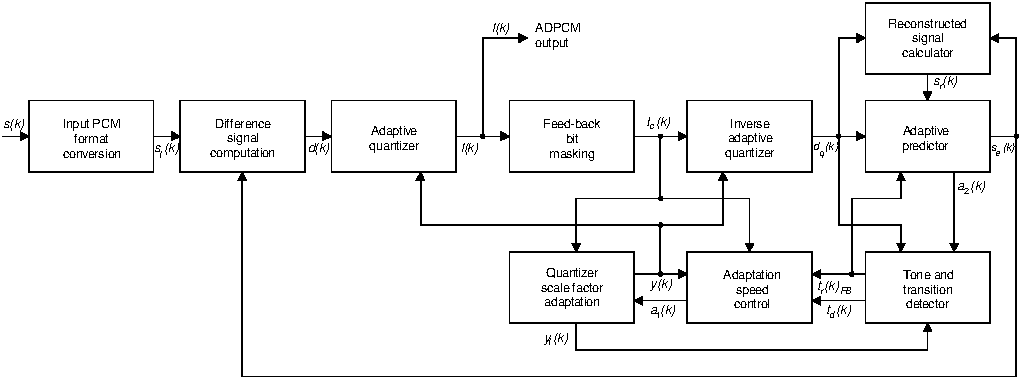
\includegraphics[scale=0.9]{g727-enc}\\

  (a) Encoder\\*[10mm]

  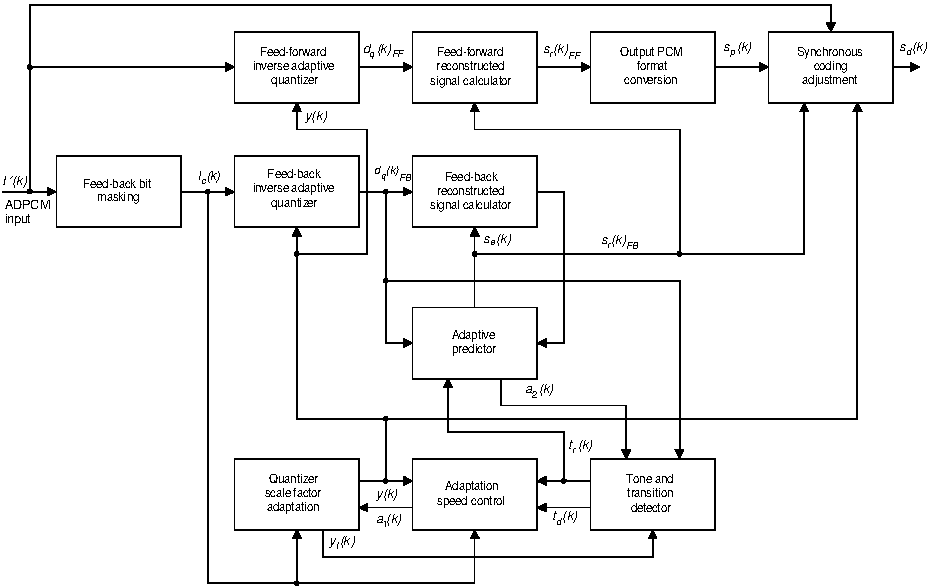
\includegraphics[scale=0.9]{g727-dec}\\

  (b) Decoder
  \end{center}

  \caption{G.727 encoder and decoder block diagrams
           \label{fig:G.727} }
\end{figure}
%-------------------------------------------------------------


\section{ITU-T STL G.727 Implementation}

The STL implementation of the G.727 algorithm can be found
in module {\tt g727.c}, with prototypes in {\tt g727.h}.

The problem of storing the state variables was solved by defining a
structure containing all the necessary variables, defining a new type
called {\tt G727\_state}. As for other STL modules, the use of the
state variable allows for parallel processing flows in the same
executable program. The internal elements of the state variable {\tt
G727\_state} should not be modified by the user, and are not described
here.

The encoding function is {\tt G727\_encode}, and the decoding function
is {\tt G727\_decode}. Additionally, initialization and reset of the
state variable is performed by {\tt g727\_reset}. There are other
internal routines which are not for access by the user, and hence are
not described here. Their usage description is given below.

\subsection{{\tt G727\_reset}}

{\bf Syntax: }

{\tt
\#include "g727.h"\\
void G727\_reset
         (\ttpbox{110mm}{
            g727\_state {\em *st});
         }
}

{\bf Prototype: }    g727.h

{\bf Description: }

  Reset ITU-T G.727 embedded ADPCM encoder or decoder state variable.


\subsection{{\tt G727\_encode}}

{\bf Syntax: }

{\tt
\#include "g727.h"\\
void G727\_encode
         (\ttpbox{110mm}{
                short {\em *src}, short {\em *dst}, short {\em smpno},
                short {\em law}, short {\em cbits}, short {\em ebits},
                g727\_state {\em *state});
         }
}

{\bf Prototype: }    g727.h

{\bf Description: }

Simulation of the ITU-T G.727 embedded ADPCM encoder. Takes the A or
$\mu$ law input array of shorts {\tt src} (16 bit, right- justified,
without sign extension) of length {\tt smpno}, and saves the encoded
samples in the array of shorts {\tt dst}, with the same number of
samples and right-justified. The ADPCM samples will have {\tt cbits}
core bits, and {\tt ebits} enhancement bits.

The state variables are saved in the structure {\em state}, which
should be initialized by {\tt g727\_reset()} before use. A-law is used
if {\em law}=={\tt '1'}, and $\mu$-law if {\em law}=={\tt '0'}.

{\bf Variables: }
\begin{Descr}{\DescrLen}
\item[\pbox{20mm}{\em src}] %\rulex{1mm}\\
               Is the input samples' buffer; each {\tt short} sample
               shall contain right-justified 8-bit wide valid A or $\mu$
               law samples.

\item[\pbox{20mm}{\em dst}] %\rulex{1mm}\\
               Buffer with right justified {\tt short} ADPCM-encoded
               samples with cbits core bits and ebits enhancement
               bits. Unused MSbs are set to zero.

\item[\pbox{20mm}{\em smpno}] %\rulex{1mm}\\
               Is a {\tt short} indicating the number of samples to encode.

\item[\pbox{20mm}{\em law}] %\rulex{1mm}\\
               Is a char indicating if the law for the input samples is A
               ({\tt '1'}) or $\mu$ ({\tt '0'}).

\item[\pbox{20mm}{\em cbits}] %\rulex{1mm}\\
               Number of core ADPCM bits.

\item[\pbox{20mm}{\em ebits}] %\rulex{1mm}\\
               Number of enhancement ADPCM bits.

\item[\pbox{20mm}{\em state}] %\rulex{1mm}\\
               The state variable structure; all the variables here are for
               internal use of the G.727 algorithm, and should not be
               changed by the user.
\end{Descr}

{\bf Return value: }        None.


\subsection{{\tt G727\_decode}}

{\bf Syntax: }

{\tt
\#include "g727.h"\\
void G727\_decode
         (\ttpbox{110mm}{
                short {\em *src}, short {\em *dst}, short {\em smpno},
                short {\em law}, short {\em cbits},
                short {\em ebits}, g727\_state {\em *state} );
         }
}

{\bf Prototype: }    g727.h

{\bf Description: }

Simulation of the ITU-T G.727 embedded ADPCM decoder. Takes the ADPCM
input array of shorts {\tt src} (16 bit, right-justified, without sign
extension) of length {\tt smpno}, and saves the decoded samples (A or
$\mu$ law) in the array of shorts {\tt dst}, with the same number of
samples and right-justified. The ADPCM samples must have {\tt cbits}
core bits, and {\tt ebits} enhancement bits.

The state variables are saved in structure {\tt st}, which should be
initialized by {\tt g727\_reset()} before use. The law is A if {\em
law}=={\tt '1'}, and $\mu$ law if {\em law}=={\tt '0'}.

{\bf Variables: }
\begin{Descr}{\DescrLen}
\item[\pbox{20mm}{\em src}] %\rulex{1mm}\\
               Buffer with right justified {\tt short} ADPCM-encoded
               samples with cbits core bits and ebits enhancement
               bits. Unused MSbs are zero.

\item[\pbox{20mm}{\em dst}] %\rulex{1mm}\\
               Is the input samples' buffer; each {\tt short} sample
               shall contain right-justified 8-bit wide valid A or $\mu$
               law samples.

\item[\pbox{20mm}{\em smpno}] %\rulex{1mm}\\
               Is a {\tt short} indicating the number of samples to encode.

\item[\pbox{20mm}{\em law}] %\rulex{1mm}\\
               Is a char indicating if the law for the input samples is A
               ({\tt '1'}) or $\mu$ ({\tt '0'}).

\item[\pbox{20mm}{\em cbits}] %\rulex{1mm}\\
               Number of core ADPCM bits.

\item[\pbox{20mm}{\em ebits}] %\rulex{1mm}\\
               Number of enhancement ADPCM bits.

\item[\pbox{20mm}{\em state}] %\rulex{1mm}\\
               The state variable structure; all the variables here are for
               internal use of the G.727 algorithm, and should not be
               changed by the user.
\end{Descr}


{\bf Return value: }        None.


%-.-.-.-.-.-.-.-.-.-.-.-.-.-.-.-.-.-.-.-.-.-.-.-.-.-.-.-.-.-.-.
\section{Portability and compliance} \label{G.727-Port}

Code testing has been done using the reset test sequences for 5, 4, 3,
and 2 bits with the valid combination of core and enhancement
bits. The reset test sequences can be acquired from the ITU Sales
Department, and are not distributed with the STL. The testing
procedure is implemented in the makefiles, which use a binary version
of the test vectors. The implementation passed the compliance test
when no differences were found between tested and reference test
vectors.  All test vectors were verified to be properly processed.

These routines have been tested in in MS-DOS with Turbo C++ v1.0
(16-bit mode) and GNU-C (go32 32-bit mode), and in Windows/32 with MS
Visual C and CYGNUS/gcc. In the Unix environment, they have been
tested for SunOs (cc, acc, and gcc), HP-UX (gcc), and Ultrix 4.0 (cc
and gcc).


\section{Example code}

%..........................................................................
\subsection {Description of the demonstration program}

One program is provided as demonstration program for the G.727 module,
g727demo.c.

Program {\tt g727demo.c} accepts input files in either 16-bit,
right-justified A- or $\mu$-law format (as generated by g711demo.c)
and encodes and/or decodes using the G.727 algorithm for the
user-specified number of $N_c$ core bits and $N_e$ enhancement
bits. The effective encoding bitrate will then be $16 \times
(N_c+N_e)$ kbit/s. Linear PCM files are not accepted by the program,
since G.727 Annex A \cite{G.727:LinearIO} is not yet implemented in
the STL. Three operations are possible: logarithmic in, logarithmic
out (default) logarithmic in, ADPCM out (option {\em -enc}), or ADPCM
in, logarithmic out (option {\em -dec}).

%..........................................................................
\subsection {Simple example}

The following C code gives an example of G.727 coding and decoding
using as input speech previously encoded by either the A- or
$\mu$-law functions available in the STL. The output samples are
encoded using the same law of the input signal.

{\tt\small
\begin{verbatim}
#include <stdio.h>
#include "ugstdemo.h"
#include "g727.h"

#define BLK_LEN 256

void main(argc, argv)
  int             argc;
  char           *argv[];
{
  G727_state      encoder_state, decoder_state;
  char            law;
  short           core, enh;
  char            FileIn[180], FileOut[180];
  short           tmp_buf[BLK_LEN], inp_buf[BLK_LEN], out_buf[BLK_LEN];
  FILE           *Fi, *Fo;

  /* Get parameters for processing */
  GET_PAR_C(1, "_Law: ......................... ", law);
  GET_PAR_I(2, "_Core bits: ................... ", core);
  GET_PAR_I(2, "_Enhancement bits: ............ ", enh);
  GET_PAR_S(2, "_Log-PCM Input File: .......... ", FileIn);
  GET_PAR_S(3, "_Log-PCM Output File: ......... ", FileOut);

  /* Opening input and output LOG-PCM files */
  Fi = fopen(FileIn, RB);
  Fo = fopen(FileOut, WB);

  /* Reset state variables */
  g727_reset(&encoder_state);
  g727_reset(&decoder_state);

  /* File processing */
  while (fread(inp_buf, BLK_LEN, sizeof(short), Fi) == BLK_LEN)
  {
    /* Process input log PCM samples in blocks of length BLK_LEN */
    G727_encode(inp_buf, tmp_buf, BLK_LEN, law, core, enh, &encoder_state);

    /* Process ADPCM samples in blocks of length BLK_LEN */
    G727_decode(tmp_buf, out_buf, BLK_LEN, law, core, enh, &decoder_state);

    /* Write PCM output word */
    fwrite(out_buf, BLK_LEN, sizeof(short), Fo);
  }

  /* Close input and output files */
  fclose(Fi);
  fclose(Fo);
}
\end{verbatim}
}
